\documentclass[12pt, titlepage]{article}

\usepackage{booktabs}
\usepackage{tabularx}
\usepackage{hyperref}
\usepackage{float}
\hypersetup{
    colorlinks,
    citecolor=black,
    filecolor=black,
    linkcolor=red,
    urlcolor=blue
}
\usepackage{graphicx}

\usepackage[round]{natbib}

\title{SE 3XA3: Requirements Document\\Genetic Cars}

\author{Team 8, Grate
		\\ Kelvin Lin (linkk4)
		\\ Eric Chaput (chaputem)
		\\ Jin Liu (liu456)
}

\date{\today}

%The follow 2 lines of code below were obtained from: 
%https://gitlab.cas.mcmaster.ca/ThisTooShallParse/3XA3_CParser/blob/master/Req_Update/L01_Group7_Requirements_Rev0.tex
\usepackage{mdframed}
\newmdenv[linecolor=black]{reqbox}


%% Comments

\usepackage{color}

\newif\ifcomments\commentstrue

\ifcomments
\newcommand{\authornote}[3]{\textcolor{#1}{[#3 ---#2]}}
\newcommand{\todo}[1]{\textcolor{red}{[TODO: #1]}}
\else
\newcommand{\authornote}[3]{}
\newcommand{\todo}[1]{}
\fi

\newcommand{\wss}[1]{\authornote{blue}{SS}{#1}}
\newcommand{\ds}[1]{\authornote{red}{DS}{#1}}
\newcommand{\mj}[1]{\authornote{red}{MSN}{#1}}
\newcommand{\cm}[1]{\authornote{red}{CM}{#1}}
\newcommand{\mh}[1]{\authornote{red}{MH}{#1}}

% team members should be added for each team, like the following
% all comments left by the TAs or the instructor should be addressed
% by a corresponding comment from the Team

\newcommand{\tm}[1]{\authornote{magenta}{Team}{#1}}


\begin{document}

\maketitle

\pagenumbering{roman}
\tableofcontents
\listoftables
\listoffigures

\begin{table}[h]
\caption{\bf Revision History}
\begin{tabularx}{\textwidth}{p{3.5cm}p{2cm}X}
\toprule {\bf Date} & {\bf Version} & {\bf Notes}\\
\midrule
October 7, 2016 & 1.0 & Started Functional Requirements\\
October 10, 2016 & 1.1 & Updated Functional Requirements\\
October 11, 2016 & 1.2 & Added Context Diagram\\
October 11, 2016 & 1.3 & Added Work Partitioning Table\\
October 11, 2016 & 1.4 & Added Off-the-Shelf Solutions\\
\bottomrule
\end{tabularx}
\end{table}

\newpage

\pagenumbering{arabic}

This document describes the requirements for ....  The template for the Software
Requirements Specification (SRS) is a subset of the Volere
template~\citep{RobertsonAndRobertson2012}.  If you make further modifications
to the template, you should explicity state what modifications were made.

\section{Project Drivers}

\subsection{The Purpose of the Project}

\subsection{The Stakeholders}

\subsubsection{The Client}

\subsubsection{The Customers}

\subsubsection{Other Stakeholders}

\subsection{Mandated Constraints}

\subsection{Naming Conventions and Terminology}

\subsection{Relevant Facts and Assumptions}

User characteristics should go under assumptions.

%KELVIN'S PART STARTS HERE
\section{Functional Requirements}

\subsection{The Scope of the Work and the Product}

\subsubsection{The Context of the Work}
The following depicts a context diagram for Grate's Genetic Cars:

\begin{figure}[h]
  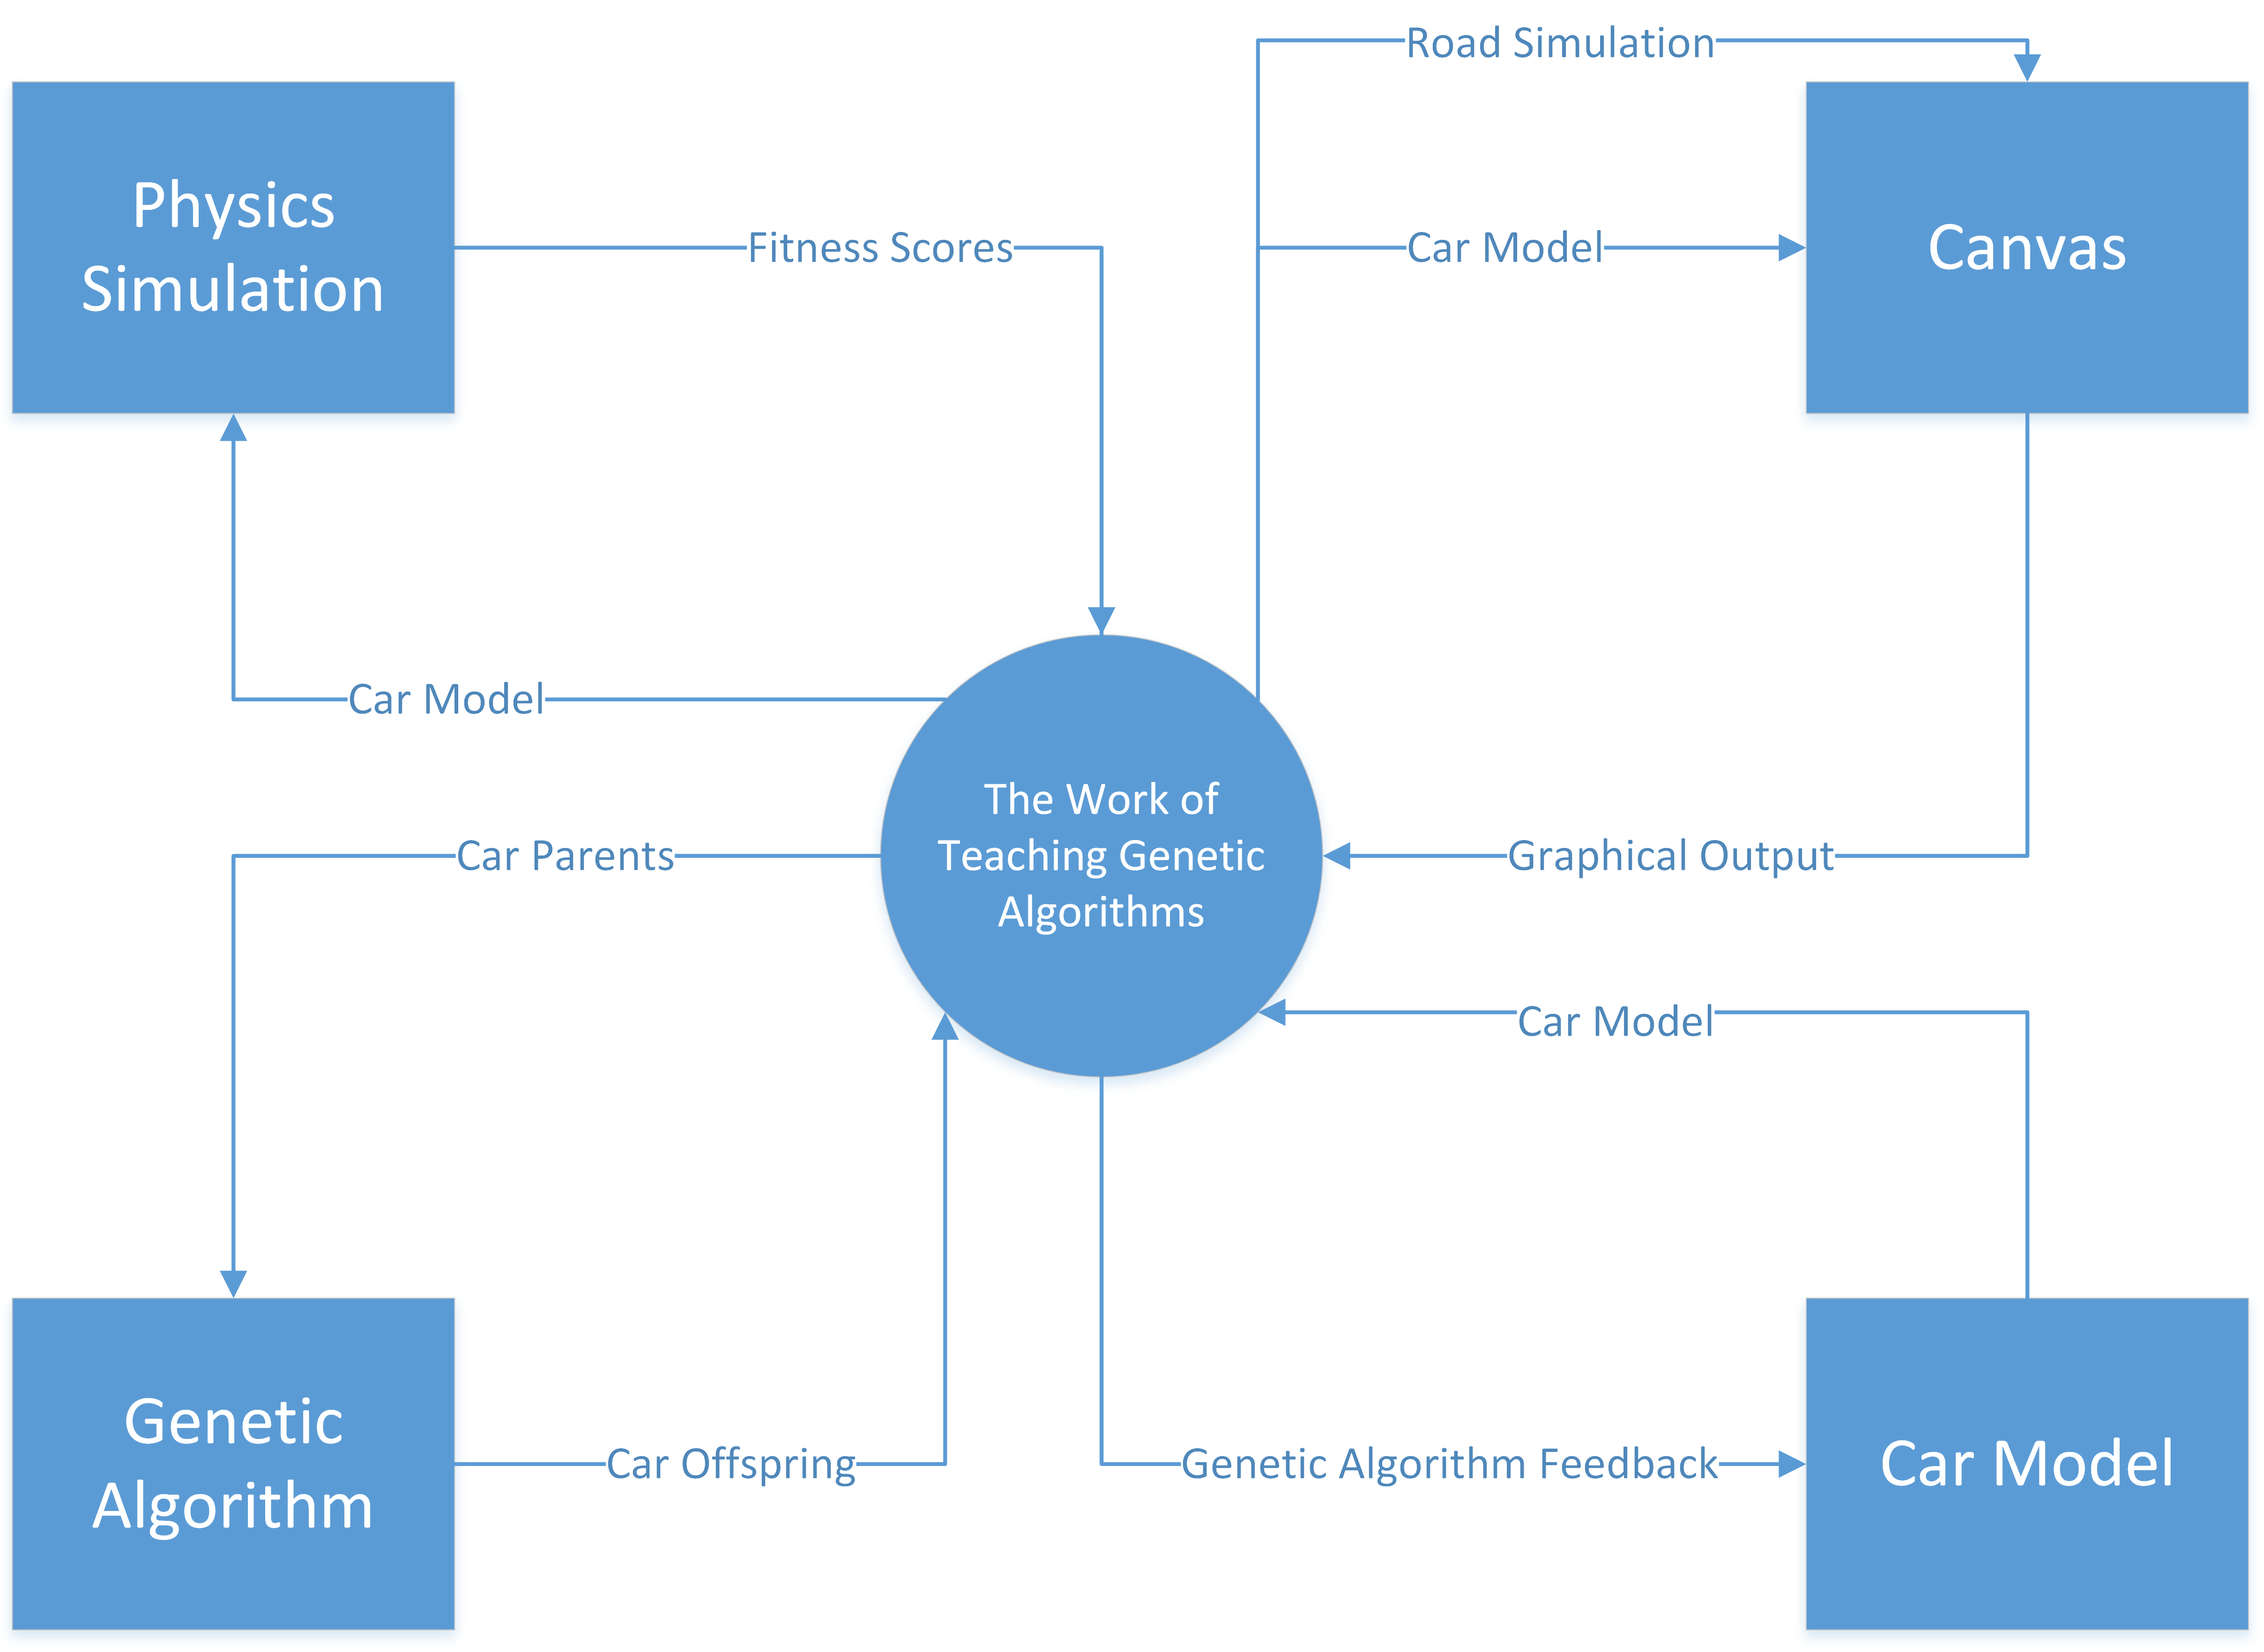
\includegraphics[width=\linewidth]{ContextDiagram.png}
  \caption{The Context Diagram for Grate's Genetic Cars}
\end{figure}

\subsubsection{Work Partitioning}
\begin{table}[H]
\begin{tabularx}{\textwidth}{p{4cm}p{4cm}X}
\toprule {\bf Event Name} & {\bf Input and Output} & {\bf Summary}\\
\midrule
1. Physics Simulation simulates generation & Car Offspring (in), Fitness Scores 
(out) & Calculate parents for the next generation\\
& & \\
2. Canvas displays car results & Car model (in), Road simulation (in), Graphical 
Display (out) & Draw car model, Track top cars, Restart at the end of the 
generation\\
& & \\
3. Genetic algorithm generates new generation & Fitness Scores (in), Car 
Offspring (out) & Selects parents from fitness scores, Cross over genes, Mutate 
genes\\
\bottomrule
\end{tabularx}
\caption{\bf Work Partitioning Table}
\end{table}

\subsubsection{Individual Product Use Cases}
\begin{enumerate}

\item{Normal Operation}

\begin{itemize}
\item{User launches program.}
\item{The Genetic Algorithm generates a random seed.}
\item{The random seed is used to generate offspring using the default 
parameters.}
\item{The Physics Simulation takes the offspring (Car Model) and performs 
physics simulations to determine their fitness score.}
\item{The results are sent to the Canvas, which displays the results 
graphically.}
\item{The fitness scores are sent back to the Genetic Algorithm to generate new 
offspring.}
\end{itemize}

\item{User Modifies Any Parameter}
\begin{itemize}
\item{User launches program.}
\item{User modifies fields in the program that pertain to the Genetic 
Algorithm's attributes.}
\item{The Genetic Algorithm generates offspring based on the user's input.}
\item{The Physics Simulation takes the offspring (Car Model) and performs 
physics simulations to determine their fitness score.}
\item{The results are sent to the Canvas, which displays the results 
graphically.}
\item{The fitness scores are sent back to the Genetic Algorithm to generate new 
offspring.}
\end{itemize}

\end{enumerate}

\subsection{Functional Requirements}

%Box formatting template adapted from: 
%https://gitlab.cas.mcmaster.ca/ThisTooShallParse/3XA3_CParser/blob/master/Req_Update/L01_Group7_Requirements_Rev0.tex





%REQUIREMENT #1
\begin{reqbox}
	%
	\begin{tabular}{cc}
		Requirement \#: 1 & Requirement Type: Functional \\
	\end{tabular} \\
	%
	\textbf{Description:} Each car must be composed of at least \textit{v} vectors. 
	\\
	\textbf{Rationale:}  This requirement manages the complexity of the car model, 
	allowing for realistic distribution of traits among members of a population. 
	That is, this prevents large cars from being generated and using an excessive 
	amount of memory. \\
	\textbf{Originator:} Kelvin Lin\\
	\textbf{Fit Criterion:} No car generated within population \textit{p} shall be 
	composed of more than \textit{v} vectors.\\
	%  
	\textbf{Supporting Materials:} JavaScript \\
	\textbf{History:} Created October 7\textsuperscript{th}, 2016
	%
\end{reqbox}

\newpage

%REQUIREMENT #2
\begin{reqbox}
	%
	\begin{tabular}{cc}
		Requirement \#: 2 & Requirement Type: Functional \\
	\end{tabular} \\
	%
	\textbf{Description:} Each car may not have more than 
	\textit{number\_of\_vertices} wheels. \\
	\textbf{Rationale:}  The wheels must be attached to the car via a vertex between 
	two connecting vectors. This requirement ensures that no redundant or unused 
	wheels will be generated.\\
	\textbf{Originator:} Kelvin Lin\\
	\textbf{Fit Criterion:} No car generated within population \textit{p} shall be 
	composed of more than \textit{number\_of\_vertices} wheels.\\
	%  
	\textbf{Supporting Materials:} JavaScript \\
	\textbf{History:} Created October 7\textsuperscript{th}, 2016
	%
\end{reqbox}

%REQUIREMENT #3
\begin{reqbox}
	%
	\begin{tabular}{cc}
		Requirement \#: 3 & Requirement Type: Functional \\
	\end{tabular} \\
	%
	\textbf{Description:} The radius of each wheel must be at most \textit{r} units. 
	\\
	\textbf{Rationale:}  This requirement manages the complexity of the car model, 
	allowing for realistic distribution of traits among members of a population. 
	That is, cars with unrealistically sized wheels will not be generated.\\
	\textbf{Originator:} Kelvin Lin\\
	\textbf{Fit Criterion:} No cars generated will have wheels with a radius larger 
	than \textit{r}.\\
	%  
	\textbf{Supporting Materials:} JavaScript \\
	\textbf{History:} Created October 7\textsuperscript{th}, 2016
	%
\end{reqbox}

\newpage

%REQUIREMENT #4
\begin{reqbox}
	%
	\begin{tabular}{cc}
		Requirement \#: 4 & Requirement Type: Functional \\
	\end{tabular} \\
	%
	\textbf{Description:} The center of each wheel generated must be attached to a 
	vertex formed by connecting vectors. \\
	\textbf{Rationale:}  Wheels cannot be floating on or around the car. This 
	requirement ensures visual coherency by requiring wheels to be attached to the 
	car model. Knowing the center of the wheel will also allow the physics engine to 
	calculate the torque and distance that the car travelled.\\
	\textbf{Originator:} Kelvin Lin\\
	\textbf{Fit Criterion:} Each wheel displayed on the screen is attached to a 
	vertex formed by connecting vectors.\\
	%  
	\textbf{Supporting Materials:} JavaScript \\
	\textbf{History:} Created October 7\textsuperscript{th}, 2016
	%
\end{reqbox}

%REQUIREMENT #5
\begin{reqbox}
	%
	\begin{tabular}{cc}
		Requirement \#: 5 & Requirement Type: Functional \\
	\end{tabular} \\
	%
	\textbf{Description:} The mass of each car must not be less than 
	\textit{min\_weight}. \\
	\textbf{Rationale:} In order to have realistic physical simulations of car 
	models, the mass of the car must have a lower limit. The lower limit will 
	guarantee the simulations to work as expected. \\
	\textbf{Originator:} Kelvin Lin\\
	\textbf{Fit Criterion:} The mass of any car models generated are greater than 
	\textit{min\_weight}.\\
	%  
	\textbf{Supporting Materials:} JavaScript \\
	\textbf{History:} Created October 10\textsuperscript{th}, 2016
	%
\end{reqbox}

\newpage

%REQUIREMENT #6
\begin{reqbox}
	%
	\begin{tabular}{cc}
		Requirement \#: 6 & Requirement Type: Functional \\
	\end{tabular} \\
	%
	\textbf{Description:} The mass of each car must not exceed \textit{max\_weight}. 
	\\
	\textbf{Rationale:} In order to have realistic physical simulations of car 
	models, the mass of each car must have an upper limit. An upper limit reduces 
	the possibility of type incompatibility with certain APIs. Additionally, it 
	ensures that the mass of each car is encoded using a known number of bits.\\
	\textbf{Originator:} Kelvin Lin\\
	\textbf{Fit Criterion:} The mass of any car models generated do not exceed 
	\textit{max\_weight}.\\
	%  
	\textbf{Supporting Materials:} JavaScript \\
	\textbf{History:} Created October 10\textsuperscript{th}, 2016
	%
\end{reqbox}

%REQUIREMENT #7
\begin{reqbox}
	%
	\begin{tabular}{cc}
		Requirement \#: 7 & Requirement Type: Functional \\
	\end{tabular} \\
	%
	\textbf{Description:} The program shall display each generation of cars 
	traversing the road. \\
	\textbf{Rationale:} The purpose of this program is to show its users the effects 
	of genetic algorithms in an interesting and engaging manner. If the program did 
	not display each generation of cars traversing the road, then the program would 
	fail in accomplishing its original objective. \\
	\textbf{Originator:} Kelvin Lin\\
	\textbf{Fit Criterion:} Each generation of cars can be seen traversing a road on 
	the medium of output.\\
	%  
	\textbf{Supporting Materials:} JavaScript \\
	\textbf{History:} Created October 10\textsuperscript{th}, 2016
	%
\end{reqbox}

\newpage

%REQUIREMENT #8
\begin{reqbox}
	%
	\begin{tabular}{cc}
		Requirement \#: 8 & Requirement Type: Functional \\
	\end{tabular} \\
	%
	\textbf{Description:} The program shall display the fitness of the top 
	\textit{n} cars. \\
	\textbf{Rationale:} The ability to compare the performance of cars during each 
	generation is useful for observing the effects of genetic algorithms because it 
	shows the users the improvement and regression of the car's performance over 
	time.\\
	\textbf{Originator:} Kelvin Lin\\
	\textbf{Fit Criterion:} A medium of output exists to provide the fitness of the 
	car on the medium of display.\\
	%  
	\textbf{Supporting Materials:} JavaScript \\
	\textbf{History:} Created October 10\textsuperscript{th}, 2016
	%
\end{reqbox}

%REQUIREMENT #9
\begin{reqbox}
	%
	\begin{tabular}{cc}
		Requirement \#: 9 & Requirement Type: Functional \\
	\end{tabular} \\
	%
	\textbf{Description:} The program shall allow the user to enter a random seed to 
	generate cars from in lieu of a randomly generated seed. \\
	\textbf{Rationale:} The ability to enter a random seed allows the results of 
	cars to be compared and to be run on multiple computers: results are not lost as 
	a result of restarting the application. \\
	\textbf{Originator:} Kelvin Lin\\
	\textbf{Fit Criterion:} The user can input a random seed into the program 
	through an input device, and the random seed is used to dictate the random 
	behaviours of the program.\\
	%  
	\textbf{Supporting Materials:} JavaScript \\
	\textbf{History:} Created October 10\textsuperscript{th}, 2016
	%
\end{reqbox}

\newpage

%REQUIREMENT #10
\begin{reqbox}
	%
	\begin{tabular}{cc}
		Requirement \#: 10 & Requirement Type: Functional \\
	\end{tabular} \\
	%
	\textbf{Description:} The user shall be allowed to modify the mutation rate, 
	\textit{mutation\_rate}. \\
	\textbf{Rationale:} Allowing the users to modify the mutation rate allows the 
	program to fulfil its objective by showing the users how the mutation rate can 
	impact the performance of the cars. \\
	\textbf{Originator:} Kelvin Lin\\
	\textbf{Fit Criterion:} The user can input a mutation rate into the program 
	through an input device, and the mutation rate is used to produce offspring in 
	the program.\\
	%  
	\textbf{Supporting Materials:} JavaScript \\
	\textbf{History:} Created October 10\textsuperscript{th}, 2016
	%
\end{reqbox}

%REQUIREMENT #11
\begin{reqbox}
	%
	\begin{tabular}{cc}
		Requirement \#: 11 & Requirement Type: Functional \\
	\end{tabular} \\
	%
	\textbf{Description:} The user shall be allowed to change the number of cars per 
	generation \textit{s} in lieu of the default value. \\
	\textbf{Rationale:} Allowing the user to change the number of cars per 
	generation \textit{s} will allow the user to see how the size of a generation 
	affects the genetic algorithm. \\
	\textbf{Originator:} Kelvin Lin\\
	\textbf{Fit Criterion:} \textit{s} is equal to the user's input for every 
	generation produced by the program.\\
	%  
	\textbf{Supporting Materials:} JavaScript \\
	\textbf{History:} Created October 10\textsuperscript{th}, 2016
	%
\end{reqbox}

\newpage

%REQUIREMENT #12
\begin{reqbox}
	%
	\begin{tabular}{cc}
		Requirement \#: 12 & Requirement Type: Functional \\
	\end{tabular} \\
	%
	\textbf{Description:} The road generated must be the same across all 
	generations. \\
	\textbf{Rationale:} Using the same road for each generation allows for 
	comparability of performance between each generation. That is, since every car 
	will traverse the same course, their fitness and performance can be compared. \\
	\textbf{Originator:} Kelvin Lin\\
	\textbf{Fit Criterion:} The road for all simulations is the same. \\
	%  
	\textbf{Supporting Materials:} JavaScript \\
	\textbf{History:} Created October 10\textsuperscript{th}, 2016
	%
\end{reqbox}

%REQUIREMENT #13
\begin{reqbox}
	%
	\begin{tabular}{cc}
		Requirement \#: 13 & Requirement Type: Functional \\
	\end{tabular} \\
	%
	\textbf{Description:} The product must generate at least \textit{s} car samples 
	per generation. \\
	\textbf{Rationale:}  GAs improve by having a large number of samples 
	(representing members in a population) intermix traits. This requirement allows 
	the GA to work by guaranteeing that a sufficient sample will be present at all 
	times.\\
	\textbf{Originator:} Kelvin Lin\\
	\textbf{Fit Criterion:} Given a user generated input, \textit{s}, the program 
	should generate \textit{s} cars for each generation.\\
	%  
	\textbf{Supporting Materials:} JavaScript \\
	\textbf{History:} Created October 7\textsuperscript{th}, 2016
	%
\end{reqbox}

\newpage

%REQUIREMENT #14
\begin{reqbox}
	%
	\begin{tabular}{cc}
		Requirement \#: 14 & Requirement Type: Functional \\
	\end{tabular} \\
	%
	\textbf{Description:} The number of cars per generation \textit{s} shall not 
	exceed \textit{max\_cars\_per\_gen}. \\
	\textbf{Rationale:} Having a maximum number of cars per generation prevents 
	memory overflow from generating too many cars per generation.\\
	\textbf{Originator:} Kelvin Lin\\
	\textbf{Fit Criterion:} The number of cars generated per generation does not 
	exceed \textit{max\_cars\_per\_gen}.\\
	%  
	\textbf{Supporting Materials:} JavaScript \\
	\textbf{History:} Created October 10\textsuperscript{th}, 2016
	%
\end{reqbox}

%REQUIREMENT #15
\begin{reqbox}
	%
	\begin{tabular}{cc}
		Requirement \#: 15 & Requirement Type: Functional \\
	\end{tabular} \\
	%
	\textbf{Description:} The program shall use the top \textit{t} cars to generate 
	offsprings. \\
	\textbf{Rationale:} The number of cars allowed to reproduce needs to be 
	specified; otherwise, no improvement can be made in car performance over the 
	generations. \\
	\textbf{Originator:} Kelvin Lin\\
	\textbf{Fit Criterion:} The parent cars of the offspring are within the top 
	\textit{t} cars.\\
	%  
	\textbf{Supporting Materials:} JavaScript \\
	\textbf{History:} Created October 10\textsuperscript{th}, 2016
	%
\end{reqbox}

\newpage

%REQUIREMENT #16
\begin{reqbox}
	%
	\begin{tabular}{cc}
		Requirement \#: 16 & Requirement Type: Functional \\
	\end{tabular} \\
	%
	\textbf{Description:} The top \textit{t} cars shall not exceed \textit{t\_max}. 
	\\
	\textbf{Rationale:} This restriction prevents \textit{t} from exceeding 
	\textit{s} or take on an unreasonable value. It ensures that the program can 
	always run by setting an upper limit to the number of cars that can reproduce in 
	a given generation. \\
	\textbf{Originator:} Kelvin Lin\\
	\textbf{Fit Criterion:} The number of cars to choose from during reproduction 
	does not exceed \textit{t\_max}.\\
	%  
	\textbf{Supporting Materials:} JavaScript \\
	\textbf{History:} Created October 10\textsuperscript{th}, 2016
	%
\end{reqbox}

%REQUIREMENT #17
\begin{reqbox}
	%
	\begin{tabular}{cc}
		Requirement \#: 17 & Requirement Type: Functional \\
	\end{tabular} \\
	%
	\textbf{Description:} The top \textit{t} cars shall not be less than 
	\textit{t\_min}. \\
	\textbf{Rationale:} This requirement ensures that there will be a sufficient 
	number of cars to produce offspring in the subsequent generations. \\
	\textbf{Originator:} Kelvin Lin\\
	\textbf{Fit Criterion:} In each generation, there are at least \textit{t\_min} 
	parents to generate offspring.\\
	%  
	\textbf{Supporting Materials:} JavaScript \\
	\textbf{History:} Created October 10\textsuperscript{th}, 2016
	%
\end{reqbox}

\newpage

%REQUIREMENT #18
\begin{reqbox}
	%
	\begin{tabular}{cc}
		Requirement \#: 18 & Requirement Type: Functional \\
	\end{tabular} \\
	%
	\textbf{Description:} A car that stalls for more than \textit{max\_secs} shall 
	be deemed non-moving. \\
	\textbf{Rationale:} A time limit needs to be imposed on the simulations in order 
	to prevent the cars from running indefinitely without making progress. \\
	\textbf{Originator:} Kelvin Lin\\
	\textbf{Fit Criterion:} All cars that say in the same spot for 
	\textit{max\_secs} are marked as non-moving and the simulation for that car is 
	stopped.\\
	%  
	\textbf{Supporting Materials:} JavaScript \\
	\textbf{History:} Created October 10\textsuperscript{th}, 2016
	%
\end{reqbox}

%REQUIREMENT #19
\begin{reqbox}
	%
	\begin{tabular}{cc}
		Requirement \#: 19 & Requirement Type: Functional \\
	\end{tabular} \\
	%
	\textbf{Description:} The fitness of a car shall not be calculated until a car 
	is deemed to be non-moving. \\
	\textbf{Rationale:} The fitness of a car is determined by distance it moves 
	during the simulation, and the simulation runs while the car is moving. 
	Therefore, the fitness of a car cannot be determined until the car is 
	non-moving. \\
	\textbf{Originator:} Kelvin Lin\\
	\textbf{Fit Criterion:} After a car is deemed non-moving, it's fitness value can 
	be assessed.\\
	%  
	\textbf{Supporting Materials:} JavaScript \\
	\textbf{History:} Created October 10\textsuperscript{th}, 2016
	%
\end{reqbox}


%REQUIREMENT #20
\begin{reqbox}
	%
	\begin{tabular}{cc}
		Requirement \#: 20 & Requirement Type: Functional \\
	\end{tabular} \\
	%
	\textbf{Description:} The user shall be able to specify \textit{t} in lieu of 
	the default value. \\
	\textbf{Rationale:} This will allow users to see the effect of changing the 
	selectivity of the genetic algorithm. \\
	\textbf{Originator:} Kelvin Lin\\
	\textbf{Fit Criterion:} In each generation, \textit{t} cars are chosen to 
	generate offspring. \\
	%  
	\textbf{Supporting Materials:} JavaScript \\
	\textbf{History:} Created October 10\textsuperscript{th}, 2016
	%
\end{reqbox}

\newpage

%KELVIN'S PART ENDS HERE

\section{Non-functional Requirements}

\subsection{Look and Feel Requirements}

As discussed in section 1.2 of this document, the users of this product include 
students and others interested in learning about genetic algorithms. With this 
in mind, the Genetic Cars project must be accessible to those without a 
background in mathematics or computer science. This accessibility begins with 
the look and feel of the project. The Genetic Cars project should appear 
aesthetically pleasing while still presenting its functions in as clean a manner 
as possible.

\subsubsection{Appearance Requirements}

The product shall be attractive to a student audience, with an emphasis on 
secondary and post-secondary students. A sampling of representative users shall, 
without prompting or enticement, be able to comprehend and use the product 
within sixty seconds of their first encounter with it. This same sampling shall 
also rate the appearance of the product on a scale from 1 to 10, and this rating 
shall be used to evaluate and refine the product's appearance. All licensing 
shall also be clear for the user to observe upon use of the product.

\subsubsection{Style Requirements}

The product shall appear inviting and educational and professional. After their 
first encounter with the product, a majority of representative users shall, 
without enticement, agree that they feel they would want to utilize the product 
and that they would learn about Genetic Algorithms by using the product. 
Representative users should also feel that they can trust the product.

\subsection{Usability and Humanity Requirements}

\subsubsection{Ease of Use Requirements}

The product shall be easy for anybody over the age of 6 to use. The product 
shall not expect the user to remember anything about the product given multiple 
uses. The product shall make the user want to use it and to show the product to 
their friends/family/etc.. The product shall be used by people with no training 
or education except for a basic knowledge of the English language and the most 
very basic functions of a computer, such as how to navigate to a web-site and 
how to enter inputs when prompted to do so. A representative sample of users 
shall be able to successfully complete a given set of tasks with the product 
within a specified period of time to be determined at the time of the sample. 
The representative sample shall also show a willingness to show the product to 
others.

\subsubsection{Personalization Requirements}

The product shall allow the user to make simple adjustments to the product to 
allow for a variable length and amount of trials depending on user input. 

\subsubsection{Learning Requirements}

The product shall be easy for an intended user of the product to learn. The 
product shall be able to be used by these users with no training before use. A 
representative sample of users shall be able to successfully complete a given 
set of tasks with the product within a specified period of time to be determined 
at the time of the sample.

\subsection{Performance Requirements}

\subsubsection{Speed and Latency Requirements}

The response time of the product shall be fast enough to avoid a loss of 
interest by the user following an input, which shall be a period of time no 
longer then five seconds. The initialization of the product shall be no longer 
then one minute.

\subsubsection{Precision and Reliability Requirements}

The product shall always converge towards a more optimal car. The product shall 
achieve 99 percent uptime. The product display shall be accurate to two decimal 
places.

\subsubsection{Longevity Requirements}

The product shall be easy to update and upgrade following its initial public 
release. 

\subsection{Operational and Environmental Requirements}

\subsubsection{Productization Requirements}

\subsection{Maintainability and Support Requirements}

\subsubsection{Maintenance Requirements}

\subsubsection{Supportability Requirements}

\subsubsection{Adaptability Requirements}

\subsection{Security Requirements}

\subsubsection{Access Requirements}

\subsubsection{Integrity Requirements}

\subsubsection{Privacy Requirements}

\subsection{Cultural Requirements}

\subsection{Legal Requirements}

\subsection{Health and Safety Requirements}

This section is not in the original Volere template, but health and safety are
issues that should be considered for every engineering project.

\section{Project Issues}

\subsection{Open Issues}
Not applicable for this project.

\subsection{Off-the-Shelf Solutions}

\subsubsection{Ready-Made Product}
Similar solutions to Grate's Genetic Cars already exists, notably BoxCar2D 
(boxcar2d.com/) and Rednuht's Genetic Cars (rednuht.org/genetic\_cars\_2/). Both 
products demonstrate the effect of genetic algorithms through evolving cars by 
selecting for the longest distance travel. They differ in that BoxCar2D displays 
one car at a time, whereas Rednuht's Genetic Cars displays all of the cars in 
one generation at once. They both allow users to adjust parameters of the 
genetic algorithm in order to observe the effects of the algorithm. They both 
show the performance of the cars over time.

\subsubsection{Reusable Components}
The Box2D API and the D3 API can both be reused in Grate's Genetic Cars. The 
Box2D API provides functionality such as Vectors and Polygons that can be used 
to model the car. The D3 API provides visualization functionality that can be 
used to visualize the performance of cars over time. These APIs provide 
functionality external to the core functionality of Grate's Genetic Cars, which 
will make them valuable assets as Grate will not have to reimplement these APIs.

\subsubsection{Products That Can Be Copied}
Rednuht's Genetic Cars is licensed under the author's custom license which 
grants others the right to reuse his code as part of their solution. 
Furthermore, both BoxCar2D and Rednuht's Genetic Cars have released their 
algorithms in some form: BoxCar2D through visuals and text, and Rednuht's 
Genetic Cars through source code. Grate's Genetic Cars can draw inspiration from 
these sources in implementing a new innovative solution to teaching genetic 
algorithms.

\subsection{New Problems}

\subsubsection{Effects on the Current Environment}
Not applicable for this project.

\subsubsection{Effects on the Installed Systems}
Not applicable for this project.

%Motivated by Nintendo's Health and Safety Documentation for the Nintendo 3DS 
%XL: 
%http://www.nintendo.com/consumer/info/en_na/docs.jsp?menu=3ds&submenu=ctr-doc-health-safety
\subsubsection{Potential User Problems}
Users may experience fatigue from prolong use of the product. Symptoms of 
fatigue can include eyestrain, dizziness, nausea, muscle pain, or general 
discomfort. To prevent fatigue, users should take periodic breaks when using the 
program for prolonged periods of time. However, fatigue should not pose a 
significant risk for this project, as the target audience for Grate's Genetic 
Cars is older teenagers and adults who have prior experience using computers and 
are  knowledgeable about the health concerns associated with prolong use of 
computers.

Users with epilepsy or prior history of seizures may also experience seizures or 
blackouts while using the product. Symptoms of seizures may include convulsions, 
eye or muscle twitching, loss of awareness, altered vision, involuntary 
movements, and disorientation. However, this risk is not significant as the risk 
of having a seizure from light flashes or patterns is low (about 1 in 4000), and 
the likelihood of experiencing a seizure can be reduced through simple steps. 
Users can reduce the risk of experience seizures while using the product if they 
sit or stand away from the screen, use the smallest screen possible, use the 
product in a well lit room, take frequent breaks, and refrain from using the 
product if tired.

\subsubsection{Limitations in the Anticipated Implementation Environment that 
May Inhibit the New Product}
Not applicable for this project.

\subsubsection{Follow-up Problems}
The implementation environment may become depreciated before the completion of 
the project, and the platforms the product is built for may no longer support 
the product after completion of implementation. This is a significant risk as 
modern programming languages and operating platforms are constantly evolving; 
however, this risk can be mitigated through writing maintainable code that can 
be converted to new standards as they arise.

\subsection{Tasks}
\subsubsection{Project Planning}


\subsubsection{Planning of the Development Phases}

\subsection{Migration to the New Product}
Not applicable for this project.

\subsection{Risks}
The Box2D API poses the most significant risk for the car model. The Box2D 
API defines the car entity in terms that can be used with many physics 
equations, which is important for calculating the fitness function of the 
car. In the event that the Box2D API proves to be infeasible for Team 8, 
alternate arrangements will have to be made in order to complete the
project: the team will resort to using basic kinematics equations to calculate 
the fitness function instead of using the API. A possible drawback to this 
approach would be that the members of Team 8 are generally unfamiliar with 
Newtonian mechanics, so external assistance would be required. 

\subsection{Costs}
There will be no cost at all since all the software (Latex editor, code 
complier etc.) and web-hosting are free. 

\subsection{User Documentation and Training}
The user documents will be simple and efficient for our project since this 
project will not ask the user to do many things. The main responsibility for 
training documentation is letting user familiar with the start button, reset 
button and output table.

\subsection{Waiting Room}
Audio effect is expected to be add to this project.

\subsection{Ideas for Solutions}
Good structure and design for this project.


\bibliographystyle{plainnat}

\bibliography{SRS}

\newpage

\section{Appendix}

%%This section has been added to the Volere template.  This is where you can 
%place additional information.

\subsection{List of Figures}

\subsection{Symbolic Parameters}

%Code Generated From http://www.tablesgenerator.com/#
\begin{table}[h!]
\centering
\label{LOF}
\begin{tabular}{ll}
Symbol & Definition \\
\textit{s} & The number of samples in a generation  \\
\textit{v} & The number of vectors in a car  \\
\textit{number\_of\_vertices} & The number of vertices formed by connecting 
vectors in a car model \\
\textit{r} & The radius of a wheel\\
\textit{min\_weight} & The minimum mass of a car\\
\textit{max\_weight} & The maximum mass of a car\\
\textit{max\_secs} & The maximum amount of time a car is allowed to stall in one 
spot\\
\textit{n} & The number of car statistics to display\\
\textit{mutation\_rate} & The rate at which genes mutate\\
\textit{max\_cars\_per\_gen} & The maximum number of cars in a given 
generation\\
\textit{t} & The number of parents in a generation\\
\textit{t\_max} & The maximum number of parents\\
\textit{t\_min} & The minimum number of parents\\
\end{tabular}
\caption{List of Figures}
\end{table}


\end{document}
